\begin{inhalt}
\renewcommand*\chapterpagestyle{scrheadings}
\chapter{Gehäuse}

Beim Gehäuse wurde wie in \ref{ref:fusion360_grundlagen} erwähnt Fussion 360 benutzt um ein Gehäuse zu Designen. Um besser ein Gehäuse zu Designen muss man ein paar Sachen vorbereiten. In diesen Fall kann man die PCB von Altium als Step datei exportiren und in Fusion hinaufladen um besser ein Gehäuse rund um die Platine zu Designen. Dafür wurde ein Spezieller Artikel benutzt (https://www.pcbway.com/blog/PCB_Design_Tutorial/3D_model_Render_with_copper_from_Altium_to_Fusion_360_.html). 

\begin{figure}[!htb]
\centering
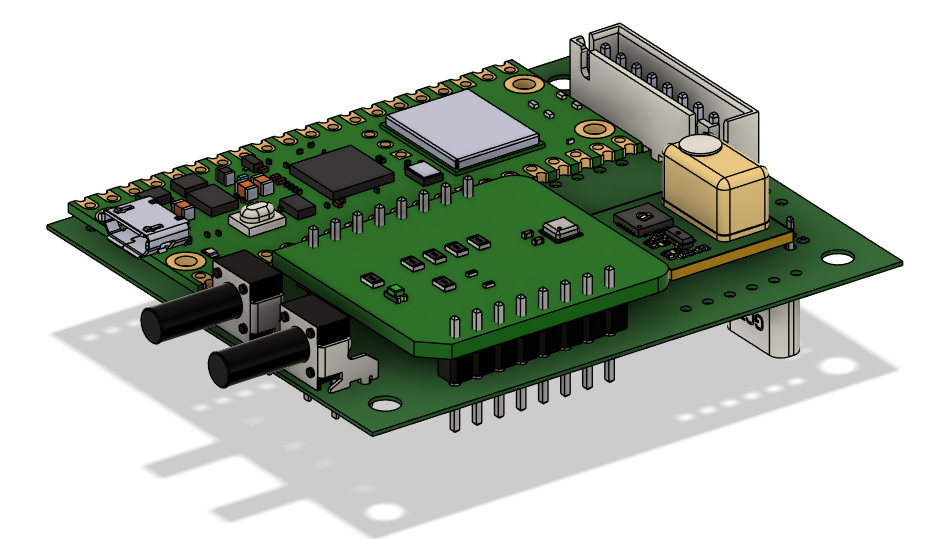
\includegraphics[width=0.75\textwidth]{files/Thomas/pics/geheause/pcb_fusion.png}
\caption[Bildbezeichnung für Abbildungsverzeichnis]{}
\label{fig:gehaeuse_internet_bild}
\end{figure}

Außerdem Wurde Das Display von hier gedownloadund und auch in das project gebracht

\begin{figure}[!htb]
\centering
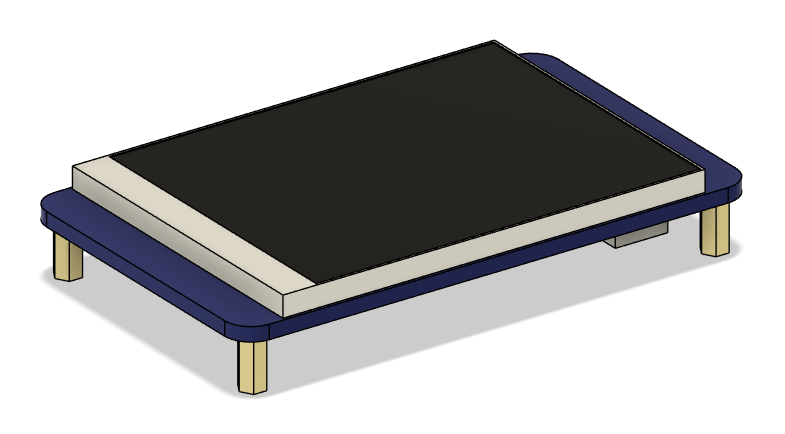
\includegraphics[width=0.75\textwidth]{files/Thomas/pics/geheause/display_fusion.png}
\caption[Bildbezeichnung für Abbildungsverzeichnis]{}
\label{fig:gehaeuse_internet_bild}
\end{figure}

Damit kann nun gestarted werden.

\subsection{Version 1.0}

\begin{figure}[!htb]
\centering
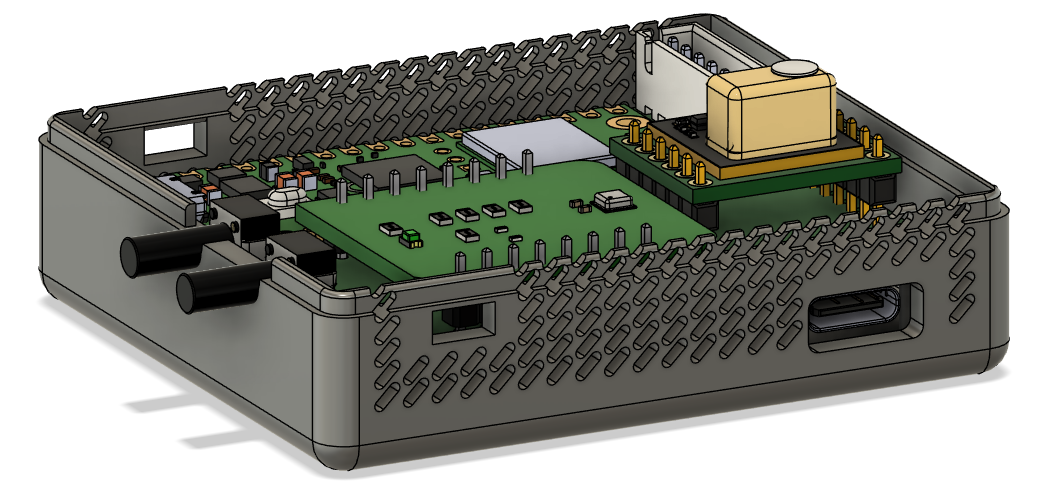
\includegraphics[width=0.75\textwidth]{files/Thomas/pics/geheause/1.0/gehaeuse_side.png}
\caption[Bildbezeichnung für Abbildungsverzeichnis]{}
\label{fig:gehaeuse_internet_bild}
\end{figure}

Bei dem ersten meilenstein gab es noch viele Probleme. Wie man in der Abbildung sehen kann war diese Version mit der Version 1.0 pcb (\ref{ref:PCB_Version_1}). Bei dieser Muste man auf den USB-C Port auf der Seite aufpassen Dieser auch sehr nahe auf der PCB dies ist schlecht da USB-C Kabel nicht genormt sind und man nie weis wie groß die Hülle ist muss man immer ein großes Loch machen Damit man mit jeden Stecker benutzen kann. Doch dieses Problem sollte bald gelöst sein.

Außer dem Wurden nur zwei clips Benutzt in der Front aber diese Waren zu wenige dieses Problem wurde auch später gelöst.

Für den Richtigen Airflow wurde das Selbe Muster wie von der Internet rechereche benutzt.

\begin{figure}[!htb]
\centering
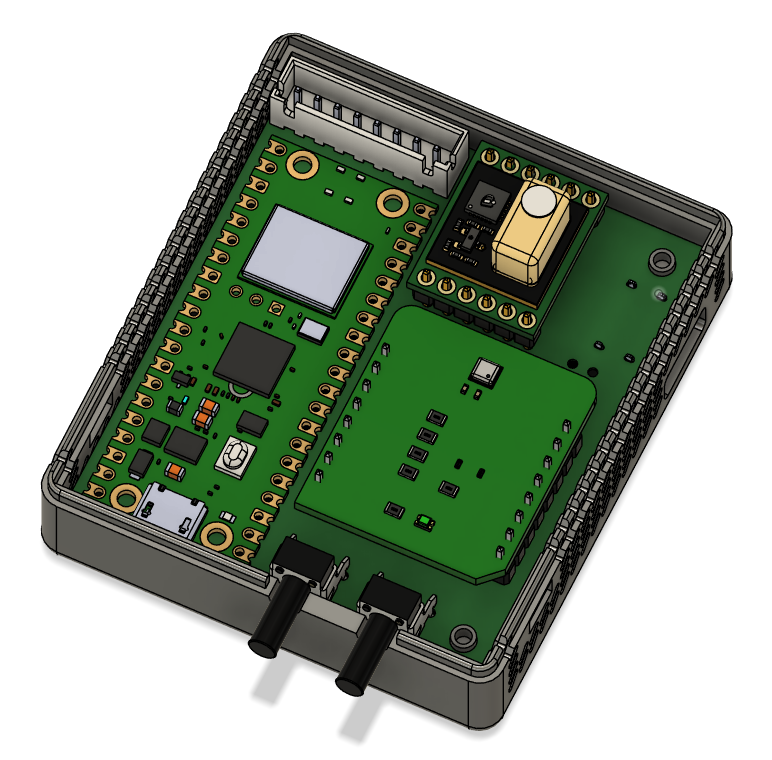
\includegraphics[width=0.75\textwidth]{files/Thomas/pics/geheause/1.0/gehaeuse_top.png}
\caption[Bildbezeichnung für Abbildungsverzeichnis]{}
\label{fig:gehaeuse_internet_bild}
\end{figure}

Wie man sehen kann ist auch bei der ersten version die Seiten Breite sehr Klein und somit brach diese Teile jedes mal ab. 

Außerdem passte beim Obriggen Teil das Display noch nicht ganz.

\newpage

\subsection{Version 1.1}

\begin{figure}[!htb]
\centering
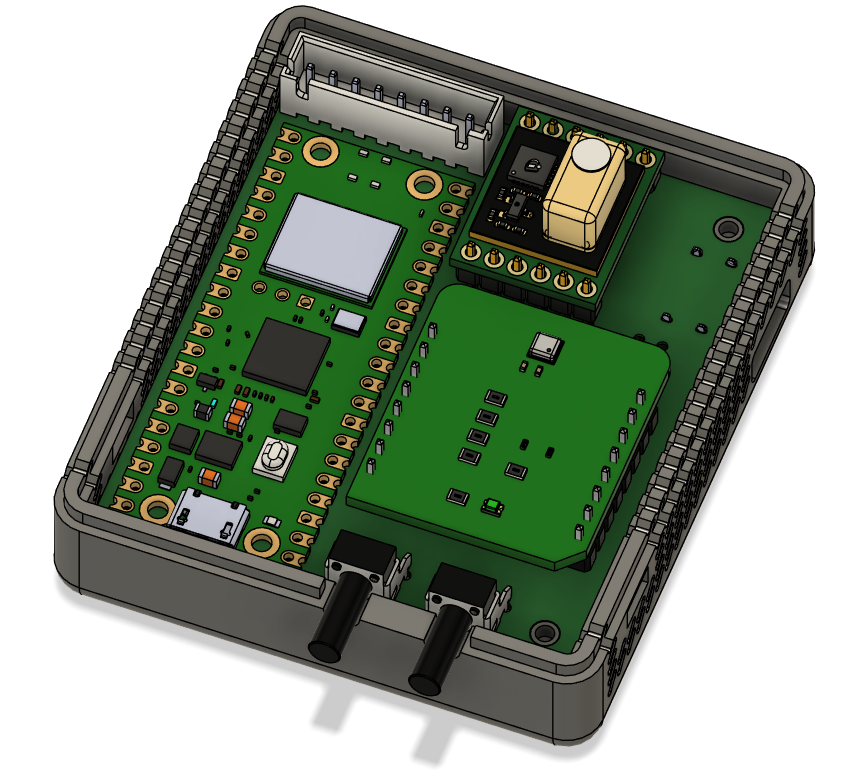
\includegraphics[width=0.75\textwidth]{files/Thomas/pics/geheause/1.1/gehaeuse_top.png}
\caption[Bildbezeichnung für Abbildungsverzeichnis]{}
\label{fig:gehaeuse_internet_bild}
\end{figure}

Der große Unterschied zwischen Version 1.0 und 1.1 ist das die Seiten vom Gehäuse Dicker geworden sind um nicht so leicht zu brechen

\subsection{Version 1.2}

\begin{figure}[!htb]
\centering
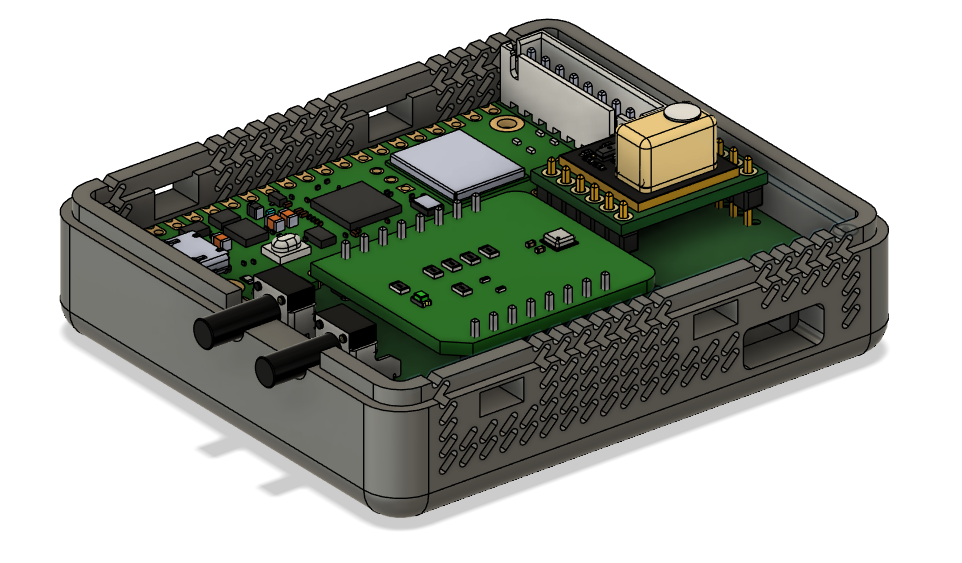
\includegraphics[width=0.75\textwidth]{files/Thomas/pics/geheause/1.2/gehaeuse_side.png}
\caption[Bildbezeichnung für Abbildungsverzeichnis]{}
\label{fig:gehaeuse_internet_bild}
\end{figure}

In dieser Version wurden 2 weitere clips hinzugefügt um das Verschliesen besser zu machen sonst würde Das gehäuse zu leicht augemacht werden

\begin{figure}[!htb]
\centering
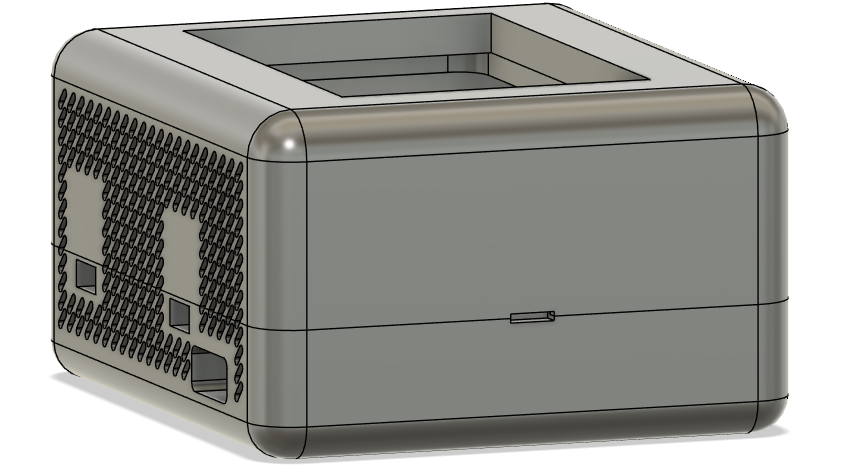
\includegraphics[width=0.75\textwidth]{files/Thomas/pics/geheause/1.2/gehaeuse_back.png}
\caption[Bildbezeichnung für Abbildungsverzeichnis]{}
\label{fig:gehaeuse_internet_bild}
\end{figure}

Außerdem wurde nun wenn das gehäuse zu stereng aufgeht ein Schlitz zwischen den Obrigen teil und den untrigen Teil gemacht um zu garantiren das man mit einen Schlitzschraufenziher das gehäuse aufzuamachen können.

Außerdem wurde die ausschneidung für das Display verbessert nun passt es perfekt in das Gehäuse mit Toleranzen und allem drum un dran


\subsection{Version 2.0}

\begin{figure}[!htb]
\centering
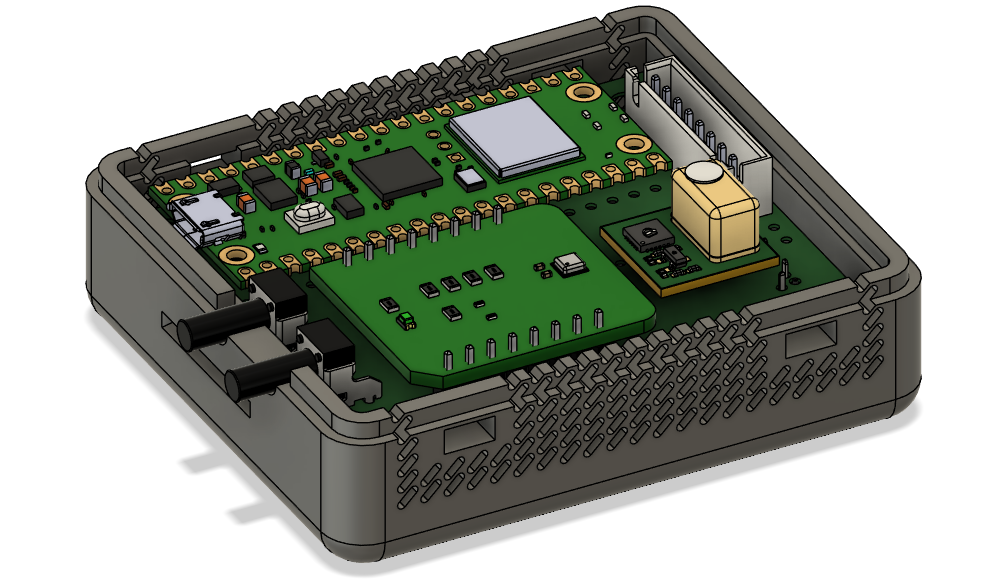
\includegraphics[width=0.75\textwidth]{files/Thomas/pics/geheause/2.0/gehaeuse_side.png}
\caption[Bildbezeichnung für Abbildungsverzeichnis]{}
\label{fig:gehaeuse_internet_bild}
\end{figure}

Da nun die PCB Version zwei (\ref{ref:PCB_Version_2}) Fertig war wurde das Gehäuse umdesigned um der PCB wieder zu passen Die wichtigsten Dinge sind da der USB-C nicht mehr auf der Seite ist kann man nun die clips Symetrisch von der Mitte gleich weit Wegplatziren damit wird noch mehr halt zwischen den Teilen versporchen.  

Außerdem wurde für das Montiren in den Kabelkanal in den Schulraume in der HTL St Pölten  kleine Sclitze gemacht die dafür sorgen das man das Geräte in den Adapter hineinstecken kann

\begin{figure}[!htb]
\centering
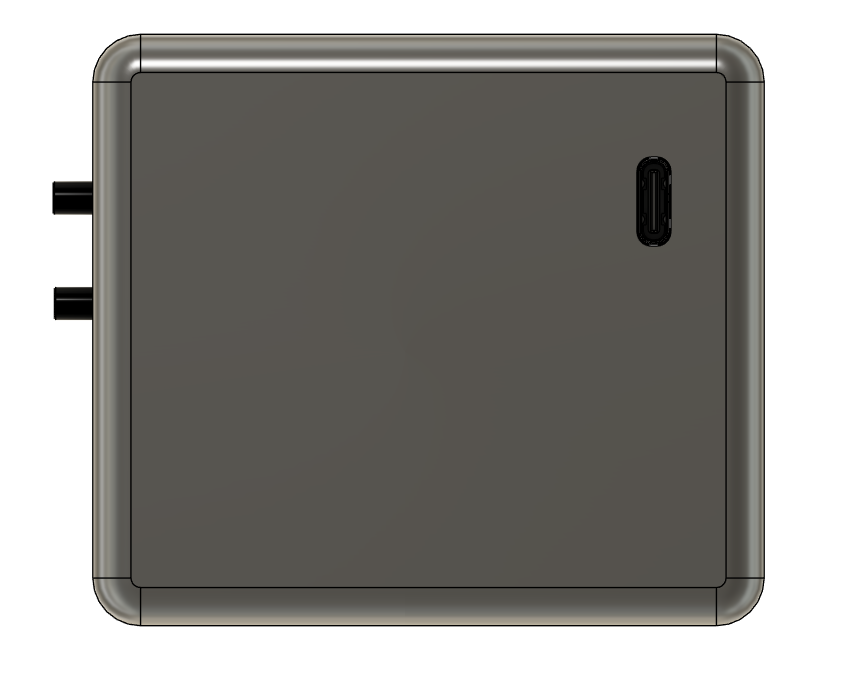
\includegraphics[width=0.75\textwidth]{files/Thomas/pics/geheause/2.0/gehaeuse_bot.png}
\caption[Bildbezeichnung für Abbildungsverzeichnis]{}
\label{fig:gehaeuse_internet_bild}
\end{figure}

Da nun der USB-C nicht merh auf der Seite ist sondern auf der Unterseite ist Ganze Thema mit USB-C gehäuse größen egal den jetzt passt jedes usb-c kabel. 

\subsection{Version 2.1}

\begin{figure}[!htb]
\centering
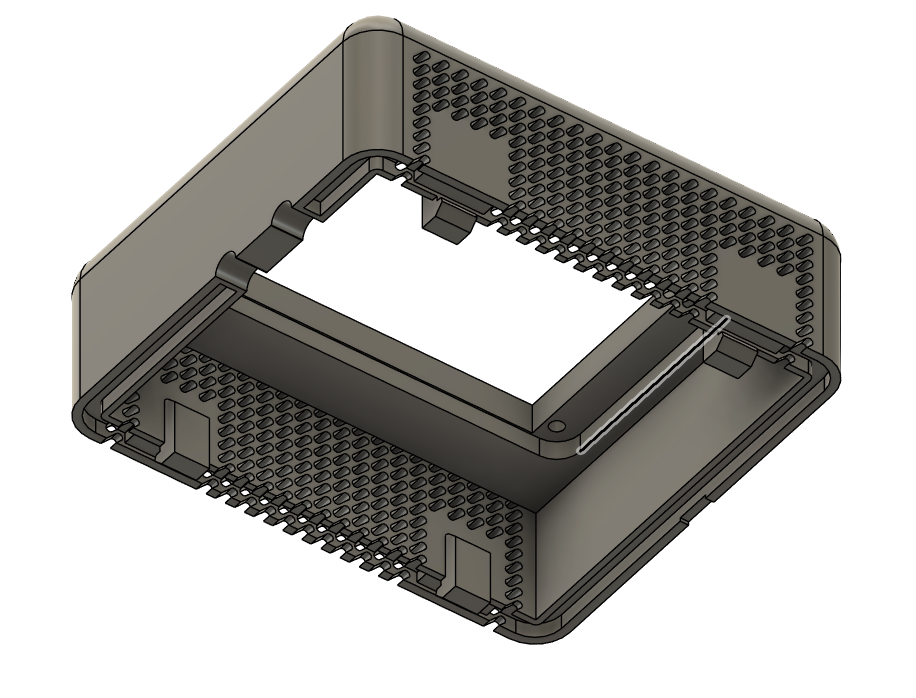
\includegraphics[width=0.75\textwidth]{files/Thomas/pics/geheause/2.1/gehaeuse_side.png}
\caption[Bildbezeichnung für Abbildungsverzeichnis]{}
\label{fig:gehaeuse_internet_bild}
\end{figure}

Da Die Clips immer wieder probleme gemacht haben wurden diesen innen Verstärkt und wurden da es probleme mit der Dicke gab verkleinert 









\end{inhalt}